% !TEX program = xelatex
% Dùng trong project template ACL (có acl.sty, acl_natbib.bst).
\documentclass[11pt]{article}
\usepackage[final]{acl}

% ── Tiếng Việt (tự nhận engine: pdfLaTeX hoặc XeLaTeX/LuaLaTeX) ──────
\usepackage{iftex}
\ifPDFTeX
  \usepackage[utf8]{inputenc}
  \usepackage[T5,T1]{fontenc}
\else
  \usepackage{fontspec}
\fi
\usepackage[vietnamese,english]{babel}

\usepackage{graphicx}
\graphicspath{{figures/}}
\usepackage{booktabs}
\usepackage{amsmath,amssymb}
\usepackage{bm}
\usepackage{multirow}
\usepackage{microtype}

\newcommand{\sys}{\textit{DataTrack}}
\newcommand{\auc}{ROC-AUC}
\newcommand{\prauc}{PR-AUC}

\title{Ứng Dụng Tư Duy Tính Toán Trong Xây Dựng Hệ Thống Gợi Ý Phỏng Vấn\\ Ngành Dữ Liệu Cá Nhân Hóa Dựa Trên Knowledge Tracing (\sys{})}

\author{
  Mai Dương Hải Đăng \quad Tạ Gia Khiêm \quad Nguyễn Sỹ Huỳnh \quad Nguyễn Ngọc Nam \\
  Trường Đại học Công nghệ Thông tin, ĐHQG-HCM \\
  \texttt{\{24520253, 24520805, 24520716, 24521114\}@gm.uit.edu.vn}
}

\begin{document}
\maketitle

\begin{abstract}
Báo cáo trình bày quá trình vận dụng \textbf{tư duy tính toán} (Computational Thinking -- CT) để xây dựng \sys{}, một hệ thống luyện phỏng vấn cá nhân hóa cho ba vai trò ngành Dữ liệu: Data Analyst (DA), Data Scientist (DS) và Data Engineer (DE), tích hợp \textbf{Knowledge Tracing} (KT). Bốn trụ cột CT---phân rã, nhận diện mẫu, trừu tượng hóa, thiết kế thuật toán---được áp dụng nhất quán: nhận diện mẫu từ bộ dữ liệu (17 Knowledge Components, learning curve, mất cân bằng lớp, rủi ro rò rỉ dữ liệu); trừu tượng hóa người học thành vector năng lực $\bm{\theta}\in[0,1]^{17}$ và lịch sử thành chuỗi $(q_t,r_t)$; thiết kế các thuật toán KT (BKT, DKT, SAKT) cùng cơ chế cập nhật năng lực và kiểm tra thích nghi. Question bank gồm 2.122 câu (snapshot 1.578 câu cho thực nghiệm) được xây bằng pipeline lai (thu thập + LLM + kiểm định); dữ liệu KT mô phỏng theo Item Response Theory gồm 1.000 người dùng và $\sim$40.000 tương tác. Trên tập kiểm tra, mọi mô hình KT vượt baseline ($\auc\approx0.68$ so với $0.50$); DKT-Quality đạt $\prauc=0.907$ và RMSE $=0.355$, tốt nhất nhóm neural. Hệ thống hoàn chỉnh (React + FastAPI + Streamlit) với chấm điểm LLM và cơ chế dự phòng cục bộ.
\end{abstract}

\section{Tổng Quan}

\subsection{Tổng quan}
Thị trường tuyển dụng IT cạnh tranh ngày càng gay gắt; theo khảo sát TopDev~\cite{topdev2024}, hơn 70\% ứng viên IT tại Việt Nam chưa chuẩn bị đủ kỹ năng trước phỏng vấn. Các nền tảng hiện có (LeetCode, HackerRank) tập trung lập trình thuật toán, thiếu nội dung cho ba vai trò ngành Dữ liệu DA/DS/DE và không theo dõi được quỹ đạo kiến thức của người học theo thời gian. Câu hỏi hiệu quả nhất là câu hơi khó hơn năng lực hiện tại---khái niệm \textit{zone of proximal development} (ZPD)~\cite{vygotsky1978mind}.

Tư duy tính toán~\cite{wing2006computational} là tập kỹ năng giúp phân tích và giải quyết vấn đề theo cách máy tính có thể thực thi, gồm bốn trụ cột: \textit{phân rã}, \textit{nhận diện mẫu}, \textit{trừu tượng hóa} và \textit{thiết kế thuật toán}. Báo cáo này vận dụng bốn trụ cột đó để trả lời câu hỏi: \textit{làm sao cá nhân hóa việc luyện phỏng vấn ngành Dữ liệu theo trình độ thực tế của từng ứng viên?} Lời giải---\sys{}---tích hợp Knowledge Tracing~\cite{corbett1994knowledge}, chấm điểm bằng mô hình ngôn ngữ lớn (LLM)~\cite{team2023gemini}, và giao diện web, được thiết kế xuyên suốt theo phương pháp CT.

\subsection{Mục tiêu nghiên cứu}
Báo cáo đặt bốn mục tiêu: (1) \textbf{nhận diện mẫu} và xây dựng bộ dữ liệu KT phù hợp cho phỏng vấn ngành Dữ liệu; (2) \textbf{trừu tượng hóa} dữ liệu thô thành biểu diễn KT chuẩn (chuỗi tương tác, vector năng lực); (3) \textbf{thiết kế thuật toán}---huấn luyện và so sánh ba họ KT (BKT, DKT, SAKT) cùng cơ chế cập nhật năng lực thời gian thực và kiểm tra thích nghi; (4) \textbf{đánh giá và tư duy phản biện}---phân tích kết quả, hạn chế và tích hợp vào ứng dụng web hoàn chỉnh.

\section{Công Trình Liên Quan}
\textbf{Knowledge Tracing.} Từ BKT~\cite{corbett1994knowledge}, các mô hình KT phát triển qua DKT~\cite{piech2015deep}, DKVMN~\cite{zhang2017dynamic}, AKT~\cite{ghosh2020context} và các mô hình Transformer như SAINT~\cite{choi2020towards}; SAKT~\cite{pandey2019self} là mô hình attention đầu tiên đơn giản mà hiệu quả. Các mô hình này được kiểm chứng chủ yếu trong môi trường học thuật (MOOC, bài tập toán, ngôn ngữ).

\textbf{Hệ thống học thích nghi.} Knewton~\cite{ferreira2017knewton} và các Intelligent Tutoring System như ASSISTments~\cite{heffernan2014assistments} dùng KT để cá nhân hóa lộ trình học, nhưng tập trung vào nội dung học thuật.

\textbf{Vị trí của \sys{}.} Khác biệt của báo cáo là áp dụng KT cho \textit{luyện phỏng vấn ngành Dữ liệu}---với câu hỏi mở, chấm điểm bằng LLM, nhiều loại câu hỏi và ba vai trò DA/DS/DE---một hướng còn ít được khai thác. Báo cáo cũng đề xuất biến thể \textit{quality label} liên tục và cơ chế blend KT--EMA cho cập nhật năng lực thời gian thực.

\section{Dữ Liệu}

\subsection{Nhận diện mẫu từ dữ liệu}
Trong \sys{}, bài toán được nhận diện là \textbf{dự đoán chuỗi}: cho lịch sử tương tác $\{(q_1,r_1),\ldots,(q_t,r_t)\}$ với $q_t$ là câu hỏi và $r_t$ là kết quả, dự đoán xác suất trả lời đúng câu kế tiếp $p(r_{t+1}=1\mid q_{t+1}, q_{1:t}, r_{1:t})$. Năng lực được theo dõi trên 17 Knowledge Components (KC) thuộc ba vai trò: DA (5 KC), DS (7 KC), DE (5 KC). Câu hỏi gồm năm loại: trắc nghiệm (MC\_SINGLE), đúng/sai (TRUE\_FALSE), điền chỗ trống (FILL\_BLANK), lý thuyết mở (THEORY) và lập trình (CODING). Dữ liệu gồm hai phần: \textit{question bank} (nội dung câu hỏi + metadata) và \textit{chuỗi tương tác} của người dùng.

\subsection{Nhận diện mẫu từ bộ dữ liệu \sys{}}
Question bank dùng cho thực nghiệm KT gồm 1.578 câu (bản triển khai mở rộng lên 2.122 câu), phủ đều ba vai trò---mỗi vai trò $\sim$500--550 câu, câu MEDIUM chiếm đa số (Hình~\ref{fig:qbank}). Bộ dữ liệu mô phỏng gồm 1.000 người dùng và 40.140 tương tác (Bảng~\ref{tab:dataset}).

\begin{figure}[t]
  \centering
  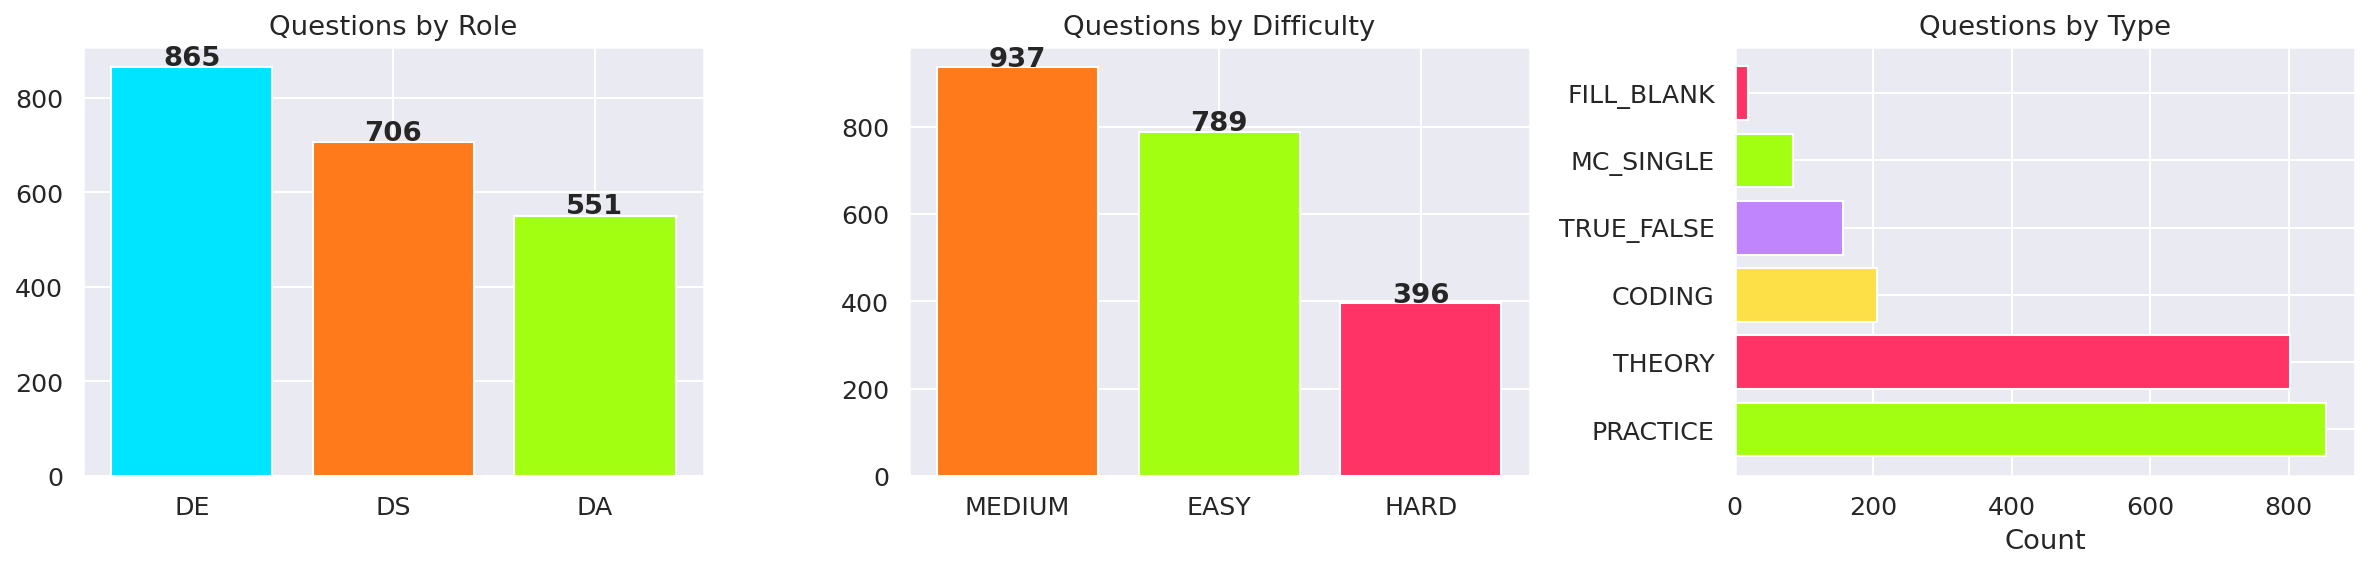
\includegraphics[width=\columnwidth]{eda_qbank_distribution.png}
  \caption{Phân bố câu hỏi theo vai trò và mức độ khó.}
  \label{fig:qbank}
\end{figure}

\begin{table}[t]
  \centering\small
  \setlength{\tabcolsep}{4pt}
  \resizebox{\columnwidth}{!}{%
  \begin{tabular}{ll}
    \toprule
    \textbf{Thuộc tính} & \textbf{Giá trị} \\
    \midrule
    Người dùng & 1.000 (DA/DS/DE = 334/333/333) \\
    Câu hỏi (snapshot KT) & 1.578 \, (triển khai: 2.122) \\
    Knowledge Components & 17 \\
    Tổng tương tác & 40.140 \, (TB 40,1/user) \\
    Train/Val/Test (theo user) & 700/150/150 \\
    Pass rate ($Q\geq1$) & 82,5\% \\
    \bottomrule
  \end{tabular}}
  \caption{Thống kê bộ dữ liệu mô phỏng.}
  \label{tab:dataset}
\end{table}

Qua phân tích khám phá (EDA), nhóm nhận diện các mẫu nổi bật: (i) \textbf{learning curve tăng đơn điệu} theo thứ tự câu hỏi (Hình~\ref{fig:lc}); (ii) \textbf{mất cân bằng lớp} với pass rate 82,5\%; (iii) \textbf{ma trận tương tác user--KC dạng block-diagonal} (mỗi user chỉ làm câu thuộc vai trò của mình), sparsity $\approx77\%$ toàn cục nhưng chỉ $15$--$20\%$ trong từng vai trò; (iv) \textbf{confidence bias}: tương quan giữa tự đánh giá và năng lực thực $r\approx0.72$; (v) phân phối trình độ thực tế beginner 40,9\%, intermediate 53,2\%, advanced 5,9\%.

\begin{figure}[t]
  \centering
  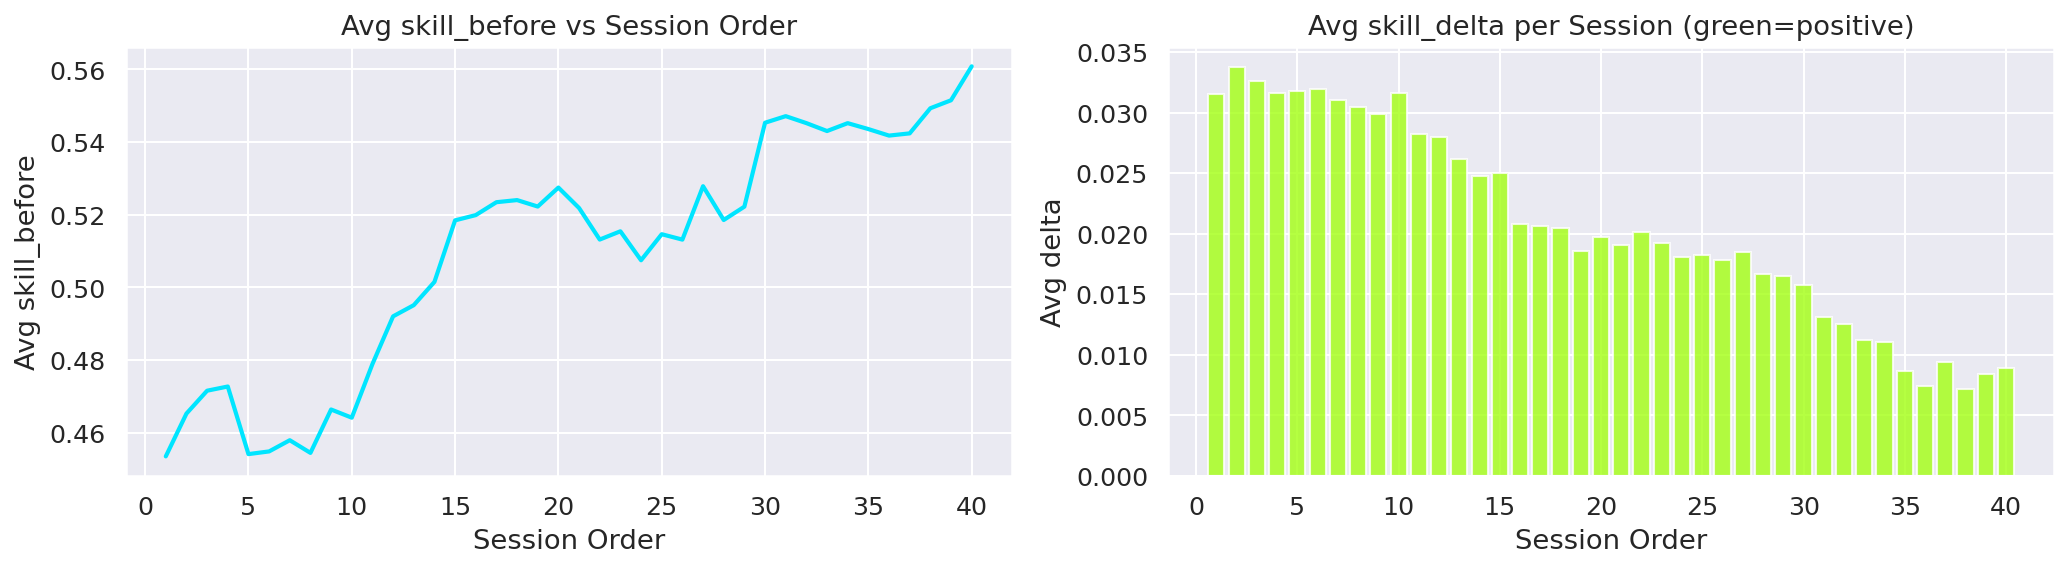
\includegraphics[width=\columnwidth]{eda_learning_curve.png}
  \caption{Learning curve: năng lực trung bình tăng theo vị trí trong chuỗi tương tác.}
  \label{fig:lc}
\end{figure}

\subsection{Liên hệ với nguyên lý tư duy tính toán}
Nguyên lý \textit{Pattern Recognition} thể hiện rõ: các mẫu quan sát được trở thành cơ sở cho mọi quyết định kỹ thuật. Cụ thể, (a) thiếu dữ liệu thật $\to$ thiết kế \textbf{pipeline mô phỏng theo IRT}; (b) bài toán có tính \textbf{chuỗi} và tương tác giữa KC $\to$ chọn mô hình KT thay vì phân loại tĩnh; (c) \textbf{mất cân bằng lớp} $\to$ dùng \prauc{} Gain thay vì chỉ Accuracy; (d) \textbf{rủi ro rò rỉ dữ liệu} (ảnh hưởng giữa các tương tác của cùng người dùng) $\to$ chia tập \textbf{theo người dùng} thay vì theo từng tương tác; (e) mẫu \textbf{cold-start} ở giai đoạn đầu $\to$ cơ chế blend KT--EMA. Như vậy, nhận diện mẫu không chỉ mô tả dữ liệu mà còn định hình toàn bộ thiết kế hệ thống.

\section{Trừu Tượng Hóa và Tiền Xử Lý Dữ Liệu}
Trong CT, trừu tượng hóa là loại bỏ chi tiết không cần thiết và xây biểu diễn có cấu trúc để máy tính xử lý hiệu quả. Mô hình KT không xử lý trực tiếp ``câu trả lời'' dạng văn bản, mà cần các biểu diễn: năng lực người học $\bm{\theta}\in[0,1]^{17}$, lịch sử dưới dạng chuỗi cặp $(q_t,r_t)$, và độ khó câu hỏi quy về tham số IRT.

\subsection{Xây dựng và chuẩn hóa question bank}
Question bank được xây qua quy trình lai bốn giai đoạn: \textbf{thu thập} từ các kho phỏng vấn công khai (Obenner cho DE, LearningZone cho SQL, các bộ DS/DA cộng đồng), có trích dẫn nguồn; \textbf{sinh tự động} bằng pipeline đa mô hình LLM~\cite{team2023gemini}---sinh câu hỏi theo KC và mức độ, tạo đáp án tham chiếu và \textit{evaluation points}; \textbf{kiểm định} (schema, đối chiếu RAG, review thủ công); và \textbf{chuẩn hóa} các tag chi tiết về 17 KC qua bảng tra \texttt{SKILL\_GROUP\_TO\_KC} (82 ánh xạ). Đây là bước trừu tượng hóa: ví dụ mọi tag \texttt{SQL\_WINDOW\_FUNCTION}, \texttt{SQL\_JOIN}, \texttt{SQL\_CTE} đều quy về KC \texttt{SQL\_DATABASE}.

\subsection{Biểu diễn dữ liệu}
Mỗi mẫu được biểu diễn dưới dạng bộ ba $(u_i, s_i, g_i)$, với $u_i$ là người dùng, $s_i=(q_t,r_t)_{t=1}^{T}$ là chuỗi tương tác, và $g_i$ là định danh người dùng (group). Vì các tương tác của cùng một người dùng phụ thuộc lẫn nhau (cùng quỹ đạo năng lực), việc đưa $g_i$ vào biểu diễn là cần thiết để tránh rò rỉ dữ liệu khi chia tập.

\subsection{Phân chia tập dữ liệu}
Để đánh giá khách quan, tập được chia \textbf{theo người dùng} (group) thay vì theo từng tương tác, đảm bảo mọi tương tác của một người chỉ thuộc một tập. Tỷ lệ $\approx70{:}15{:}15$ (Bảng~\ref{tab:split}); kiểm tra xác nhận không người dùng nào xuất hiện ở nhiều tập, hạn chế rò rỉ.

\begin{table}[t]
  \centering\small
  \begin{tabular}{lrr}
    \toprule
    \textbf{Tập} & \textbf{Người dùng} & \textbf{Tương tác} \\
    \midrule
    Train & 700 & 28.164 \\
    Validation & 150 & 5.911 \\
    Test & 150 & 6.065 \\
    \bottomrule
  \end{tabular}
  \caption{Phân chia dữ liệu theo người dùng.}
  \label{tab:split}
\end{table}

\subsection{Kiểm tra tính toàn vẹn dữ liệu}
Trước khi huấn luyện, bộ dữ liệu được xác thực qua bảy tiêu chí: (1) \textit{data leakage}---không người dùng nào xuất hiện ở cả train lẫn test; (2) \textit{label distribution}---pass rate train (82,7\%) $\approx$ test (82,2\%), chênh $<1\%$; (3) \textit{sequence length} trung bình 40, phân phối đều; (4) \textit{KC frequency drift}---2/17 KC lệch $>3\%$ (KC~0: 3,9\%; KC~3: 3,5\%); (5) \textit{class imbalance} 82,5\% (do đó dùng \prauc{}); (6) \textit{quality distribution} đều trong $[0,1]$; (7) \textit{cold-start coverage} 100\% người dùng. Các kiểm tra này hiện thực nguyên lý CT về xác thực dữ liệu trước khi xử lý.

\subsection{Mô phỏng tương tác bằng IRT}
Do thiếu dữ liệu thật, hành vi người dùng được trừu tượng hóa bằng Item Response Theory~\cite{embretson2000item}. Người dùng ảo được sinh với skill vector phân phối Gaussian có tương quan giữa các KC liên quan. Xác suất trả lời đúng theo IRT $P(\text{đúng})=\sigma((\theta-b)\times6)$; điểm chất lượng theo mô hình bậc (power-based graded response, $\alpha=2.0$): $P(Q{=}2)=p^{\alpha}$, $P(Q{=}0)=(1-p)^{\alpha}$; năng lực cập nhật $\theta\mathrel{+}=\eta(1-\theta)$ khi đúng, $\theta\mathrel{-}=\gamma\theta$ khi sai ($\eta=0.08$, $\gamma=0.002$, seed 42).

\subsection{Chuẩn hóa toán học}
Độ khó EASY/MEDIUM/HARD ánh xạ thành $b\in\{0.30,0.55,0.80\}$. Nhãn được biểu diễn ở hai dạng: nhị phân $r_t\in\{0,1\}$ và \textit{quality label} liên tục $r_t\in[0,1]$. Chuỗi tương tác được mã hóa thành tensor đầu vào cho DKT/SAKT---hoàn tất việc chuyển dữ liệu thô thành bài toán học máy chuẩn.

\section{Thiết Kế Thuật Toán}

\subsection{Mô hình Knowledge Tracing}
\textbf{BKT}~\cite{corbett1994knowledge} mô hình mỗi KC bằng chuỗi Markov ẩn hai trạng thái với bốn tham số $P(L_0),P(T),P(S),P(G)$; xác suất đúng $P(r_t{=}1)=P(L_t)(1{-}P(S))+(1{-}P(L_t))P(G)$, cập nhật theo Bayes. \textbf{DKT}~\cite{piech2015deep} dùng LSTM~\cite{hochreiter1997long}: $\mathbf{h}_t=\text{LSTM}(\mathbf{x}_t,\mathbf{h}_{t-1})$, $\hat{y}_{t+1}=\sigma(\mathbf{W}\mathbf{h}_t+\mathbf{b})$. Nhóm mở rộng \textbf{DKT-Quality} với nhãn liên tục và mất mát MSE: $\mathcal{L}=\frac{1}{T}\sum_t (r_t-\hat{y}_t)^2$. \textbf{SAKT}~\cite{pandey2019self} thay LSTM bằng self-attention~\cite{vaswani2017attention}, song song hóa tốt và diễn giải được attention.

\subsection{Thuật toán cập nhật năng lực (EMA + Blend)}
Để xử lý cold-start, năng lực được cập nhật thời gian thực bằng trung bình trượt mũ (EMA) rồi blend với KT:
\begin{equation}
\theta^{\text{EMA}}_t=\alpha s_t+(1-\alpha)\theta^{\text{EMA}}_{t-1},\;\alpha=0.35,
\end{equation}
\begin{equation}
\hat{\theta}_t=\lambda\,\theta^{\text{KT}}_t+(1-\lambda)\,\theta^{\text{EMA}}_t,\;\lambda=0.70,
\label{eq:blend}
\end{equation}
trong đó KT chỉ tham gia khi lịch sử $\geq3$ tương tác. EMA (trọng số 0,3) ổn định hóa dự đoán ở giai đoạn đầu; KT (0,7) nắm động lực chuỗi. Hằng số được giữ nhất quán giữa backend và frontend để con số hiển thị đồng bộ.

\subsection{Thuật toán kiểm tra thích nghi (MST)}
Phiên đánh giá dùng Computerized Adaptive Testing hai giai đoạn~\cite{wainer2000computerized}: \textbf{Stage 1} chọn câu phủ đều các KC để định vị; điểm trung bình quyết định phân nhánh WEAK/MID/STRONG. \textbf{Stage 2} chọn câu chuyên sâu, ưu tiên KC yếu nhất, độ khó điều chỉnh theo nhánh. Vector năng lực cập nhật theo từng trục KC bằng cùng pipeline EMA--Blend (Công thức~\ref{eq:blend}).

\subsection{Engine gợi ý theo ZPD}
Câu hỏi được xếp hạng theo điểm tổng hợp ưu tiên KC yếu:
\begin{equation}
\text{score}(q)=0.65\,w + 0.30\,d + 0.05\,c,
\end{equation}
với $w$ là mức yếu của KC ($w=\max(0,0.40-\theta_{kc})/0.40$), $d$ là độ phù hợp độ khó với năng lực (chiến lược ZPD), $c$ là độ phủ KC. Ngưỡng KC yếu/mạnh là $0.40/0.70$.

\subsection{Ý nghĩa của quá trình thiết kế}
Từ góc độ CT, thiết kế đã \textbf{phân rã} bài toán thành pipeline gồm các bước rõ ràng (sinh dữ liệu $\to$ huấn luyện $\to$ blend $\to$ gợi ý), và \textbf{trừu tượng hóa} mô hình KT thành ánh xạ $f(\text{lịch sử};\bm{\theta})\to\bm{m}$ với $\bm{m}$ là mức thành thạo 17 KC. Việc đề xuất quality label minh họa khả năng chuyển một \textit{nhận định ở mức bài toán} (điểm số mang nhiều thông tin hơn nhãn đúng/sai) thành một \textit{cơ chế tính toán cụ thể} (đổi BCE sang MSE).

\section{Đánh Giá, Kiểm Thử và Tư Duy Phản Biện}

\subsection{Môi trường và cấu hình}
Quy trình KT offline được tổ chức thành bốn notebook chạy tuần tự---EDA $\to$ feature engineering $\to$ huấn luyện $\to$ đánh giá---mỗi bước nhận đầu ra của bước trước, cố định seed 42 để tái lập. Thực nghiệm chạy trên Kaggle (GPU Tesla T4, PyTorch~\cite{pytorch2019} 2.6). Ablation study gồm 8 cấu hình: Baseline, BKT, DKT-Binary, DKT-Quality$^\star$, SAKT-Binary, SAKT-Quality$^\star$, DKT-Deep, SAKT-Deep. Mô hình neural dùng dropout~\cite{srivastava2014dropout}, batch 64, 30 epoch, early stopping. Do mất cân bằng lớp 82,5\%, \prauc{} Gain là chỉ số so sánh chính.

\subsection{Kết quả}
Bảng~\ref{tab:results} và Hình~\ref{fig:ablation} cho thấy mọi mô hình KT vượt baseline ($\auc$ 0.67--0.68; \prauc{} Gain 0.083--0.087).

\begin{table*}[t]
  \centering\small
  \begin{tabular}{lrrrrrr}
    \toprule
    \textbf{Mô hình} & \textbf{\auc} & \textbf{\prauc} & \textbf{\prauc{} Gain} & \textbf{RMSE} & \textbf{Acc} & \textbf{Thời gian (s)} \\
    \midrule
    Baseline            & 0.500 & 0.820 & 0.000 & 0.384 & 0.820 & 0.0 \\
    BKT                 & \textbf{0.677} & 0.905 & 0.085 & 0.374 & 0.820 & 61.9 \\
    DKT-Binary          & 0.666 & 0.905 & 0.085 & 0.375 & 0.822 & 30.8 \\
    DKT-Quality$^\star$ & 0.672 & \textbf{0.907} & \textbf{0.087} & \textbf{0.355} & 0.796 & 20.9 \\
    SAKT-Binary         & 0.668 & 0.903 & 0.083 & 0.373 & 0.822 & \textbf{11.3} \\
    SAKT-Quality$^\star$& 0.667 & 0.904 & 0.084 & 0.356 & 0.776 & 12.0 \\
    DKT-Deep            & 0.669 & 0.906 & 0.086 & 0.375 & 0.822 & 116.4 \\
    SAKT-Deep           & 0.670 & 0.906 & 0.086 & 0.373 & 0.822 & 31.4 \\
    \bottomrule
  \end{tabular}
  \caption{Kết quả ablation study trên tập kiểm tra (150 người dùng, 6.065 tương tác). $^\star$: dùng quality label liên tục.}
  \label{tab:results}
\end{table*}

\begin{figure}[t]
  \centering
  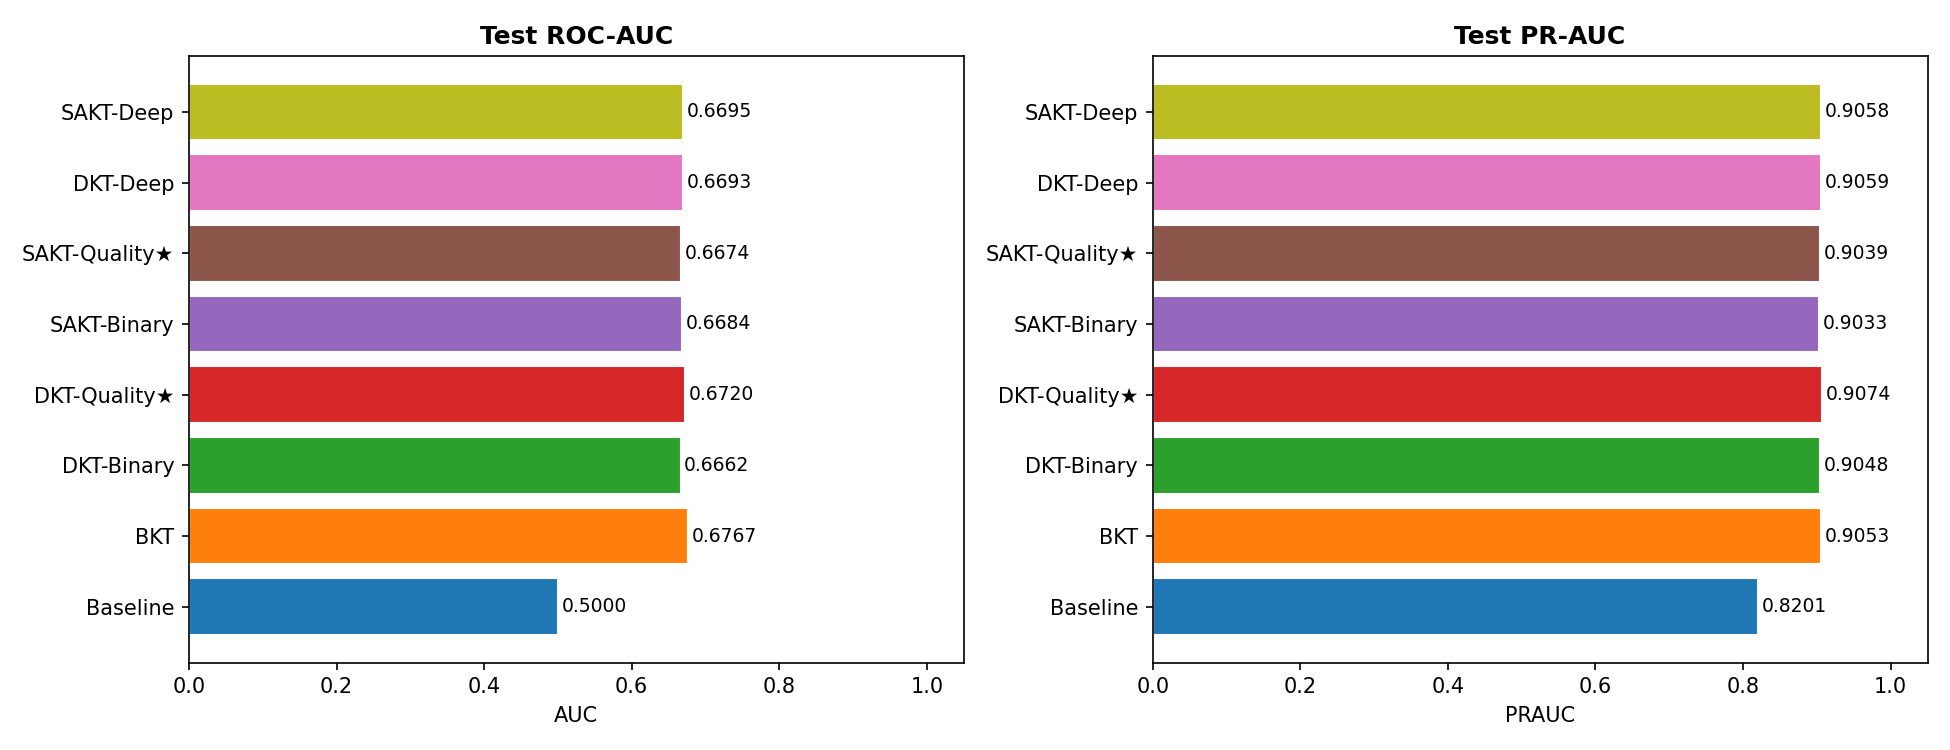
\includegraphics[width=\columnwidth]{ablation_bar.png}
  \caption{So sánh \auc{} và \prauc{} của 8 cấu hình.}
  \label{fig:ablation}
\end{figure}

\subsection{Phân tích kết quả}
\textbf{Quality label.} DKT-Quality$^\star$ đạt \prauc{} cao nhất (0.907) và RMSE thấp nhất (0.355), vượt DKT-Binary; nhãn liên tục cung cấp gradient phong phú hơn. Accuracy thấp hơn do tối ưu MSE thay vì cross-entropy.
\textbf{Simulation bias.} BKT đạt \auc{} cao nhất (0.677) vì dữ liệu sinh theo IRT---cùng dạng tham số per-KC với BKT---tạo lợi thế không công bằng; trên dữ liệu thật, mô hình neural dự kiến tốt hơn.
\textbf{Deep model.} Bản deep không cải thiện đáng kể nhưng tốn thời gian gấp nhiều lần: nút thắt là kích thước dữ liệu (28K tương tác), không phải kiến trúc.

\subsection{Phân tích sâu và tư duy phản biện}
Phân tích phân tầng (Hình~\ref{fig:perkc},~\ref{fig:err}) làm rõ năm khía cạnh. \textbf{Theo KC:} hiệu suất không đồng đều---các KC tần suất thấp (KC~0 \texttt{SQL\_DATABASE} và KC~3, drift $3{,}5$--$3{,}9\%$) có \auc{} thấp hơn; DKT-Quality$^\star$ vượt BKT ở đa số KC của DS/DE, còn BKT cạnh tranh hơn ở KC của DA (skill DA phân bố đơn giản, hợp với dạng tham số per-KC của BKT). \textbf{Theo vị trí chuỗi:} \auc{} tăng từ đầu (0--25\%) đến cuối chuỗi (75--100\%)---càng nhiều lịch sử, dự đoán càng tốt. \textbf{Theo độ khó:} câu MEDIUM có \auc{} cao nhất (vùng phân biệt mạnh của IRT); EASY chịu ảnh hưởng class imbalance, HARD ít dữ liệu. \textbf{Theo loại người dùng:} nhóm intermediate dễ dự đoán nhất nhờ phân phối đúng/sai cân bằng hơn. \textbf{Cold-start:} tương quan dương yếu giữa cold-start score và per-user \auc{}, cho thấy self-rating mang thông tin bổ sung nhưng không phải yếu tố duy nhất. Phân tích lỗi cho thấy mô hình thiên về dự đoán Pass (False Negative $>$ False Positive) do mất cân bằng lớp. Những quan sát này thể hiện tư duy phản biện: một phần kết quả tốt đến từ thiên lệch mô phỏng, nên cần kiểm chứng trên dữ liệu thật.

\begin{figure}[t]
  \centering
  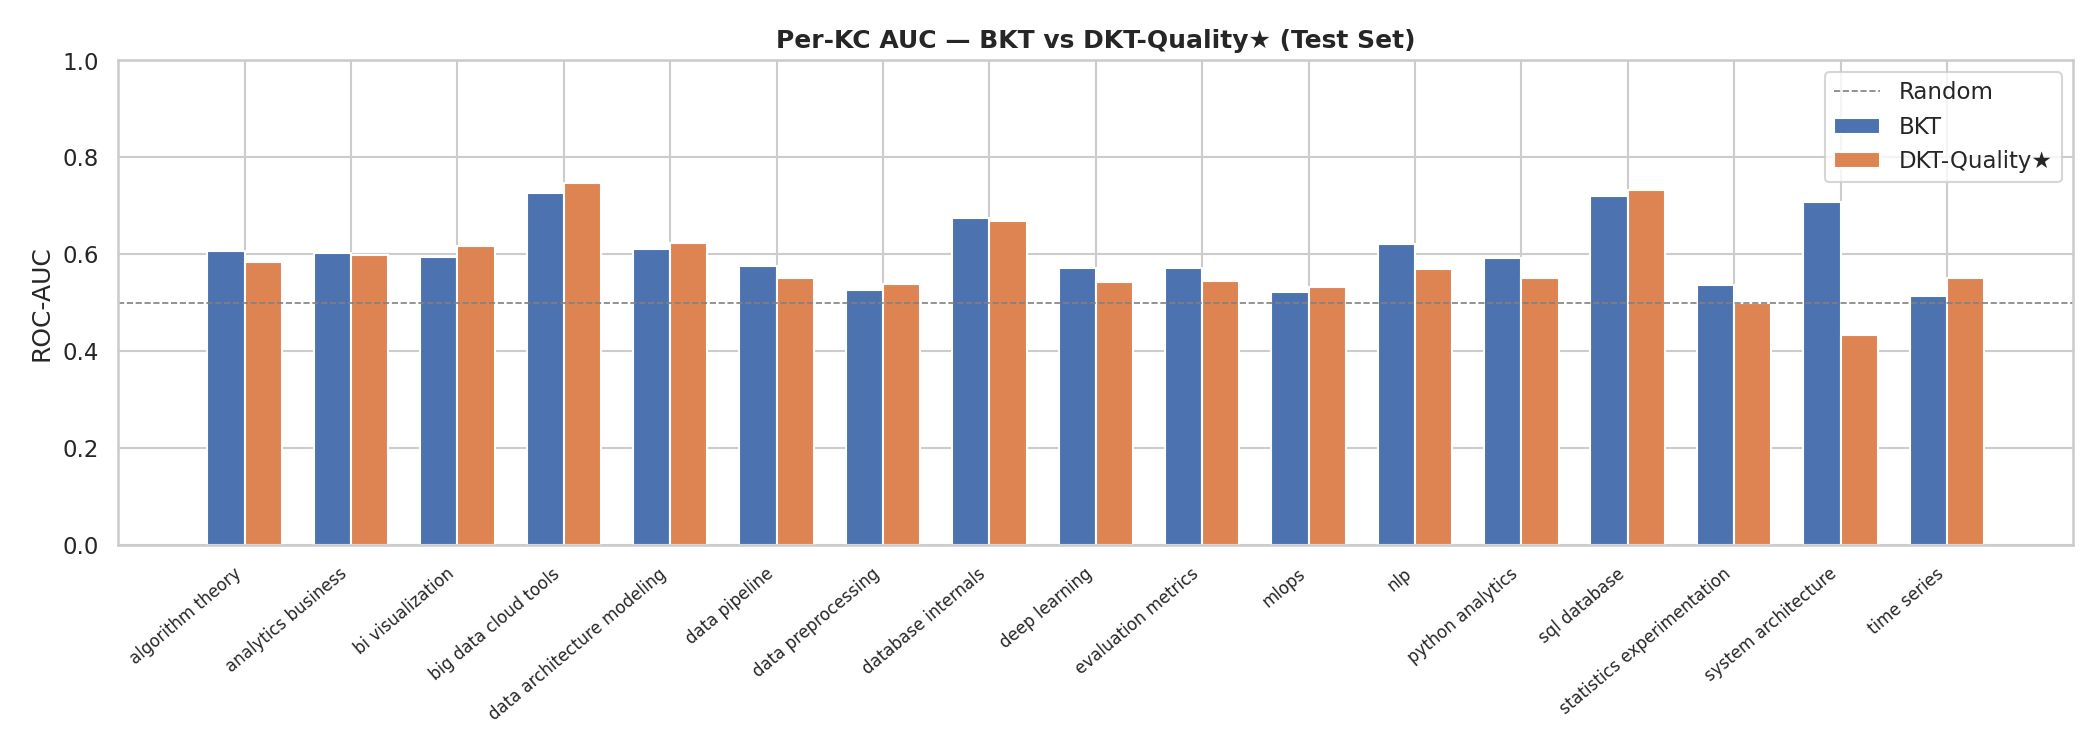
\includegraphics[width=\columnwidth]{per_kc_auc.png}
  \caption{\auc{} theo từng KC: BKT vs DKT-Quality$^\star$.}
  \label{fig:perkc}
\end{figure}

\begin{figure}[t]
  \centering
  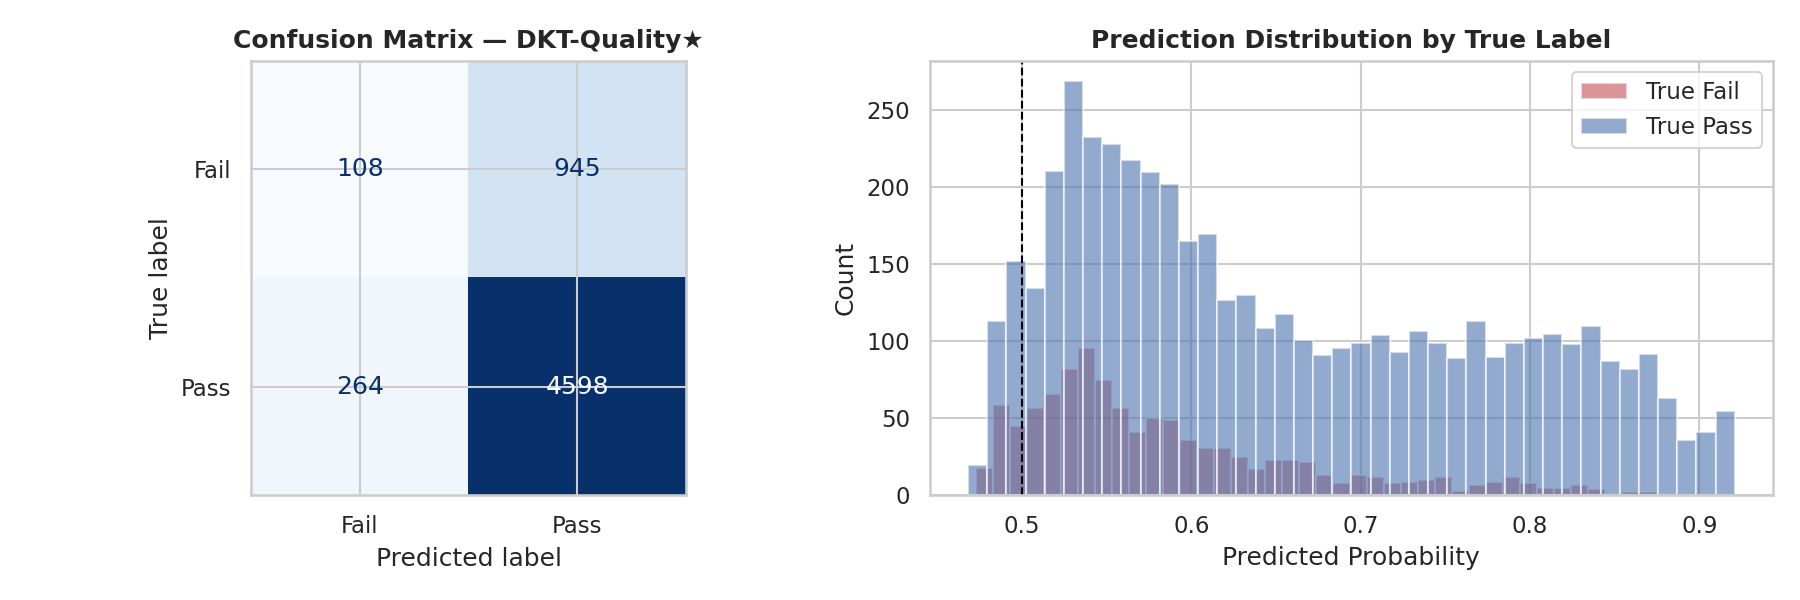
\includegraphics[width=\columnwidth]{error_analysis.png}
  \caption{Confusion matrix và phân phối điểm dự đoán---DKT-Quality$^\star$.}
  \label{fig:err}
\end{figure}

\subsection{Hệ thống ứng dụng}
DKT-Quality$^\star$ được chọn làm mô hình triển khai vì dự đoán cả 17 KC trong một forward pass, phù hợp gợi ý thời gian thực. Hệ thống tổ chức thành ba tầng. \textbf{Tầng dữ liệu} chuẩn hóa question bank và ánh xạ \texttt{skill\_groups} về 17 KC qua Competency Engine. \textbf{Tầng KT/scoring} nạp mô hình tốt nhất ở runtime, chạy pipeline EMA--Blend (Công thức~\ref{eq:blend}) và chấm điểm. \textbf{Tầng phục vụ} gồm FastAPI (9 endpoint), Streamlit làm host và React SPA; FastAPI được tách khỏi Streamlit để phục vụ tĩnh đúng MIME type và gọi API độc lập. Câu khách quan chấm tất định; câu tự luận/coding chấm bằng Gemini~\cite{team2023gemini} theo rubric, lui về local rubric khi LLM lỗi (một \textit{evaluation point} ``đạt'' khi $\geq50\%$ từ khóa xuất hiện). Toàn bộ luồng onboarding $\to$ kiểm tra thích nghi (MST hai giai đoạn) $\to$ chấm điểm $\to$ cập nhật năng lực $\to$ dashboard hoạt động end-to-end.

\section{Kết Luận}
Báo cáo đã vận dụng đầy đủ bốn trụ cột tư duy tính toán để xây dựng \sys{}: nhận diện mẫu từ bộ dữ liệu, trừu tượng hóa người học thành chuỗi tương tác và vector năng lực, thiết kế các thuật toán KT cùng cơ chế cập nhật/gợi ý, và đánh giá có phản biện. Kết quả xác nhận KT mang lại giá trị thực ($\auc\approx0.68$ so với 0.50), với DKT-Quality tốt nhất nhóm neural.

\subsection{Hạn chế}
\textbf{Simulation bias} (nghiêm trọng nhất): dữ liệu IRT tạo lợi thế cho BKT, cần dữ liệu thật để kiểm chứng. \textbf{Sequence length cố định} 40 do pool câu mỗi vai trò bị cap, làm mô hình không học được chuỗi dài/ngắn khác nhau. \textbf{Mất cân bằng lớp} (pass rate $\approx82\%$) làm \prauc{} bị inflate; \prauc{} Gain đáng tin hơn để so sánh. \textbf{KC frequency imbalance} (nhẹ): 2/17 KC lệch tần suất train/test $>3\%$, khắc phục bằng stratified split theo KC. \textbf{Data scale} (nhẹ): $\sim$28K tương tác train chưa đủ để khai thác mô hình sâu. \textbf{Phân phối trình độ lệch} (advanced chỉ 5,9\%) và \textbf{phụ thuộc LLM} khi chấm câu mở---chưa calibrate với human annotation.

\subsection{Hướng phát triển}
Thu thập dữ liệu thật và A/B test; tích hợp forgetting curve~\cite{ebbinghaus1885memory} và spaced repetition~\cite{wozniak1990optimization}; thử AKT~\cite{ghosh2020context}/SAINT~\cite{choi2020towards} khi đủ dữ liệu; mở rộng question bank và triển khai production.

\section*{Lời cảm ơn}
Nhóm xin cảm ơn giảng viên môn Tư duy tính toán và quý thầy cô Trường Đại học Công nghệ Thông tin, ĐHQG-HCM đã hướng dẫn và hỗ trợ trong quá trình thực hiện.

\begin{thebibliography}{99}
\bibitem{wing2006computational} J.~M. Wing. 2006. Computational thinking. \textit{Communications of the ACM}, 49(3):33--35.
\bibitem{vygotsky1978mind} L.~S. Vygotsky. 1978. \textit{Mind in Society}. Harvard University Press.
\bibitem{topdev2024} TopDev. 2024. Vietnam IT Market Report 2024. Technical report.
\bibitem{corbett1994knowledge} A.~T. Corbett and J.~R. Anderson. 1994. Knowledge tracing: Modeling the acquisition of procedural knowledge. \textit{User Modeling and User-Adapted Interaction}, 4(4):253--278.
\bibitem{piech2015deep} C.~Piech et al. 2015. Deep knowledge tracing. In \textit{NeurIPS}, volume~28.
\bibitem{pandey2019self} S.~Pandey and G.~Karypis. 2019. A self-attentive model for knowledge tracing. In \textit{Proc. EDM}.
\bibitem{hochreiter1997long} S.~Hochreiter and J.~Schmidhuber. 1997. Long short-term memory. \textit{Neural Computation}, 9(8):1735--1780.
\bibitem{vaswani2017attention} A.~Vaswani et al. 2017. Attention is all you need. In \textit{NeurIPS}.
\bibitem{embretson2000item} S.~E. Embretson and S.~P. Reise. 2000. \textit{Item Response Theory for Psychologists}. Lawrence Erlbaum.
\bibitem{wainer2000computerized} H.~Wainer et al. 2000. \textit{Computerized Adaptive Testing: A Primer}, 2nd ed. Lawrence Erlbaum.
\bibitem{srivastava2014dropout} N.~Srivastava et al. 2014. Dropout: A simple way to prevent neural networks from overfitting. \textit{JMLR}, 15(56):1929--1958.
\bibitem{ghosh2020context} A.~Ghosh, N.~Heffernan, and A.~S. Lan. 2020. Context-aware attentive knowledge tracing. In \textit{ACM SIGKDD}.
\bibitem{choi2020towards} Y.~Choi et al. 2020. Towards an appropriate query, key, and value computation for knowledge tracing. In \textit{ACM L@S}.
\bibitem{zhang2017dynamic} J.~Zhang, X.~Shi, I.~King, and D.-Y. Yeung. 2017. Dynamic key-value memory networks for knowledge tracing. In \textit{Proc. WWW}, pages 765--774.
\bibitem{ferreira2017knewton} P.~Ferreira. 2017. Knewton's adaptive learning platform. White Paper, Knewton Inc.
\bibitem{heffernan2014assistments} N.~T. Heffernan and C.~L. Heffernan. 2014. The ASSISTments ecosystem. \textit{International Journal of Artificial Intelligence in Education}, 24(4):470--497.
\bibitem{team2023gemini} Gemini Team, Google. 2023. Gemini: A family of highly capable multimodal models. arXiv:2312.11805.
\bibitem{pytorch2019} A.~Paszke et al. 2019. PyTorch: An imperative style, high-performance deep learning library. In \textit{NeurIPS}.
\bibitem{ebbinghaus1885memory} H.~Ebbinghaus. 1885. \textit{Memory: A Contribution to Experimental Psychology}.
\bibitem{wozniak1990optimization} P.~A. Wozniak and E.~J. Gorzelanczyk. 1990. Optimization of repetition spacing in the practice of learning. \textit{Acta Neurobiologiae Experimentalis}, 54:59--62.
\end{thebibliography}

\end{document}
